\chapter{“人在环中”的外骨骼优化}

数十年来,科研人员提出了各式各样的控制算法,但无一例外地需要根据穿戴者去精心的调节各种参数,这些参数的调整多以经验和试错为主,并没有严格的标准。以BLEEX下肢外骨骼系统为例,BLEEX所使用的灵敏度放大算法非常依赖精确的动力学模型,针对不同的穿戴者需要设计不同的灵敏度放大系数,并通过不断试错的方式来得到最合适的参数。

由于人类个体之间生理学与神经学的差异,每个人都有其偏好的行走习惯和行走模式,对外骨骼不同助力模式的感受不尽相同,不同个体对同一助力模式的反应也大相径庭。只有为穿戴者提供最适合的助力模式,才能真正的实现有效辅助与人体机能提升。因此,寻找适合穿戴者的助力模式是一项非常有挑战性的工作。

\begin{figure}[!htb]
    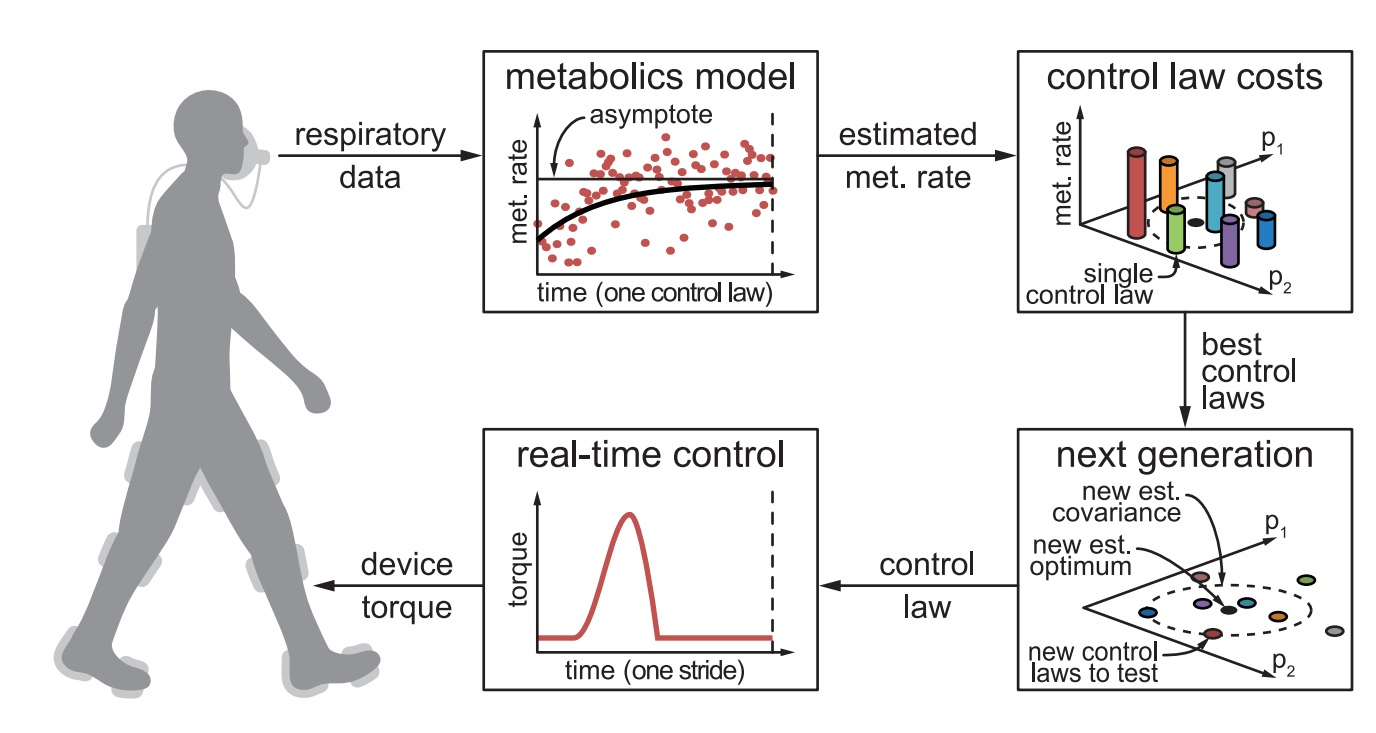
\includegraphics[width=15cm]{fig/f60.jpg}
    \caption{“人在环中”的优化方法\cite{p40}}
    \label{fig:mark}
\end{figure}

“人在环中”的优化方法正是在这种背景下被提出。针对不同的个体,根据其对助力模式反应,在助力行走过程中实时的调整助力参数,以达到为穿戴者提供最佳的助力模式,这种方法被称为“人在环中”的优化方法。在这种方法中,穿戴者成为外骨骼系统环路的一部分,为助力参数的选择提供反馈信息,如图4.1所示。
\begin{align}
    p^{*} & = \mathop{min}\limits_{p} f(p) \\
    f(p):\quad &p \to adaptedness
\end{align}

“人在环中”的优化方法把调整助力参数的过程看做是一个优化问题,其中适应度为助力参数的函数,通过优化适应度函数的最小值来得到穿戴者最适合的助力参数。然而适应度函数并不是一个具有显示表达的目标函数,也不是一个可以描述的确定过程,而是穿戴者在与外骨骼交互的过程中产生的一个生理信号。由于人体生理及运动过程太过复杂,无法进行建模,所以适应度函数是未知的,只能通过实时的采样得到。因此“人在环中”的优化本质上是一个黑箱优化,而且是一个目标函数采样困难、含有噪声的黑箱优化问题。

任何一个足够复杂的系统都可以视为黑箱模型。研究人员探索了许多用于黑箱优化的算法\cite{p48},如随机搜索、遗传算法、模拟退火、单纯形法、贝叶斯优化等等。但由于进行“人在环中”优化时,人体的生理反馈信号含有巨大的噪声,因此很多方法并不适用。在现有的研究成果中,协方差矩阵自适应进化策略\cite{p40}(CMA-ES)和贝叶斯优化\cite{p41}(BO),已被证明是两种可行的方案。

本章针对“人在环中”的优化问题,使用人体肌肉活跃度为生理反馈,通过贝叶斯优化的方法对上层控制的两个控制参数进行优化,在20次迭代内完成最优参数的辨识。

\section{贝叶斯优化}

贝叶斯优化的核心为贝叶斯定理:
\begin{align}
    p(f|D_{1:t})=\frac{D_{1:t}|p(f)}{p(D_{1:t})}
\end{align}

其中$f$表示位置的目标函数,$D_{1:t} = \{(x_1,y_1),\cdots,(x_t,y_t)\}$表示既有数据集;$p(D_{1:t}|f)$为数据集中观测量的似然分布,反应了观测数据的噪声;$p(f)$表示$f$的先验概率分布,即对前一步对目标函数的估计;$p(f|D_{1:t}$表示$f$的后验分布,即在观测后对目标函数的更新估计。

贝叶斯优化是一种序贯优化方法,它在每一次对目标函数采样后,主动选择下一个合理的参数进行采样,从而尽快的达到最优解。本质上来说,贝叶斯优化通过利用历史信息,用代理模型拟合真实目标,根据对拟合模型的估计,产生一个“最有意义”的采样点,不断迭代从而实现快速而高效的优化。

贝叶斯优化主要由两部分组成:用于拟合观测数据的概率代理模型和产生新采样点的采集函数。本文所使用的概率代理模型和采集函数分别为高斯过程模型和LCB采集函数。

高斯过程(GP)是一种常用的非参数模型,用以对未知目标函数进行拟合,广泛应用在回归、分类等领域。高斯过程由一个均值函数和一个协方差函数构成:
\begin{align}
    f(x)\sim \mathcal{GP}(m(x),k(x,x'))
\end{align}

由Sherman-Morrison-Woodbury公式\cite{p49}可得,在数据集为$D_{1:t} = \{(x_1,y_1),\cdots,(x_t,y_t)\}$时,高斯过程可表示为:
\begin{align}
    P(f|D_{1:t},x) &= N(\mu_t(x),\sigma^2(x)) \\
    \mu_t(x) &= \mathbf{k}^T\mathbf{K}^{-1}\mathbf{f}_{1:t} \\
    \sigma^2(x) &= k(\mathbf{x},\mathbf{x}) - \mathbf{k}^T\mathbf{K}^{-1}\mathbf{k}
\end{align}

其中
\begin{align}
\mathbf{K} & =\left[ \begin{array}{ccc}{k\left(\mathbf{x}_{1}, \mathbf{x}_{1}\right)} & {\dots} & {k\left(\mathbf{x}_{1}, \mathbf{x}_{t}\right)} \\ {\vdots} & {\ddots} & {\vdots} \\ {k\left(\mathbf{x}_{t}, \mathbf{x}_{1}\right)} & {\dots} & {k\left(\mathbf{x}_{t}, \mathbf{x}_{t}\right)}\end{array}\right] \\
\mathbf{k}&=\left[k\left(\mathbf{x}, \mathbf{x}_{1}\right) \quad k\left(\mathbf{x}, \mathbf{x}_{2}\right) \quad \cdots \quad k\left(\mathbf{x}, \mathbf{x}_{t}\right)\right] \\
k &\left(\mathbf{x}_{i}, \mathbf{x}_{j}\right)=\exp \left(-\frac{1}{2}\left\|\mathbf{x}_{i}-\mathbf{x}_{j}\right\|^{2}\right)
\end{align}

采集函数用来选择下一次优化迭代的采样点。在进行采样点选取时,有两个基本的出发点:
\begin{enumerate}
    \item 对均值函数最小值处进行采样,提高对最优参数估计精度
    \item 对方差函数最大值处进行采样,以降低模型估计的不确定度
\end{enumerate}

前者表示对模型的利用,后者表示对模型位置的探索。任何一种采样函数都需要在探索和利用之间进行权衡,使得优化算法能够得到较高精度的全局最优解。其中LCB方法就是其中一种典型的采集函数:
\begin{align}
    LCB(x) = \mu(x) - k\sigma(x)
\end{align}

超参数$k$用来调节探索与利用之间的比重,$k$越大则越倾向于对未知进行探索。通过求取函数$LCB(x)$的最小值,即可得到下一次优化迭代需要采样的参数。

\begin{algorithm}[h]
    \caption{贝叶斯优化}
    \begin{algorithmic}[1]
    \FOR{$i = 1,2,\cdots$}
    \STATE 最小化高斯过程的采集函数,得到采样参数:$x_t=\mathop{min}\limits_{x}LCB(x)$\
    \STATE 对目标函数进行采样:$y_t = f(x_t)+\epsilon_t$\
    \STATE 更新高斯过程:$D_{1:t} = \{ D_{1:t-1},(x_t,y_t)\}$
    \ENDFOR
    \end{algorithmic}
\end{algorithm}

贝叶斯优化的算法流程如上所示,每一次迭代开始时当前对目标函数估计的高斯过程,计算采集函数的最小值,得到本次迭代的参数,之后对目标函数进行采样,最后用观测到的数据更新高斯过程。贝叶斯优化可以看做是一个具有想象力的算法,它从已有数据想象出目标函数的大致形状,并选择有价值的点进行采样,以调整自己的想象,使得估计的参数不断地向最优参数靠近并收敛。

\section{基于肌肉激活指标的生理反馈信号}

为了实现“人在环中”优化,必须要选择合适的人体生理信号进行反馈,目前使用较多的反馈信号为人体的代谢耗能,但代谢耗能数据获取较为困难,需要两分钟才能完成一次目标函数的采样,时间成本较高。因此本文选择人体肌电信号作为生理反馈。
\begin{figure}[htb]
    \subfloat[步态过程关节力矩]{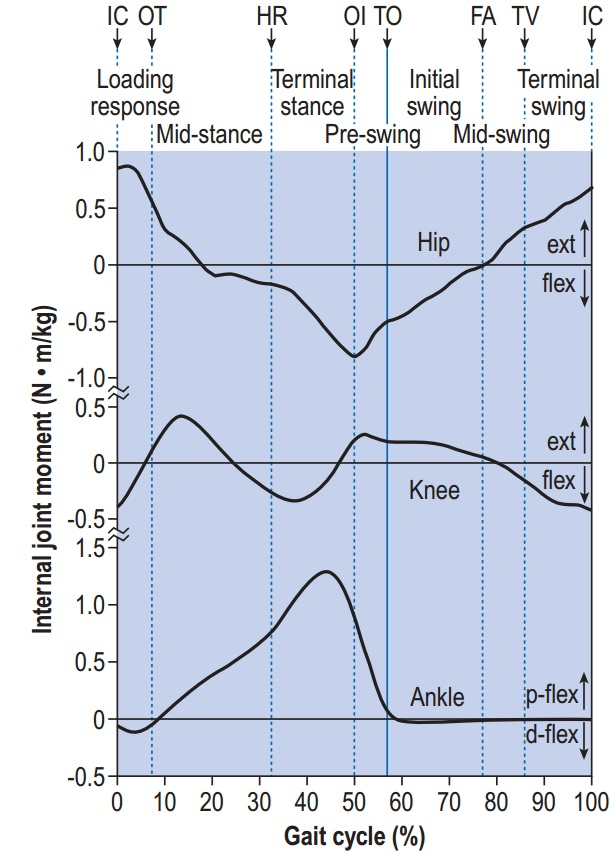
\includegraphics[width=8.9cm]{fig/f52.jpg}}
    \subfloat[步态过程腿部肌肉激活度]{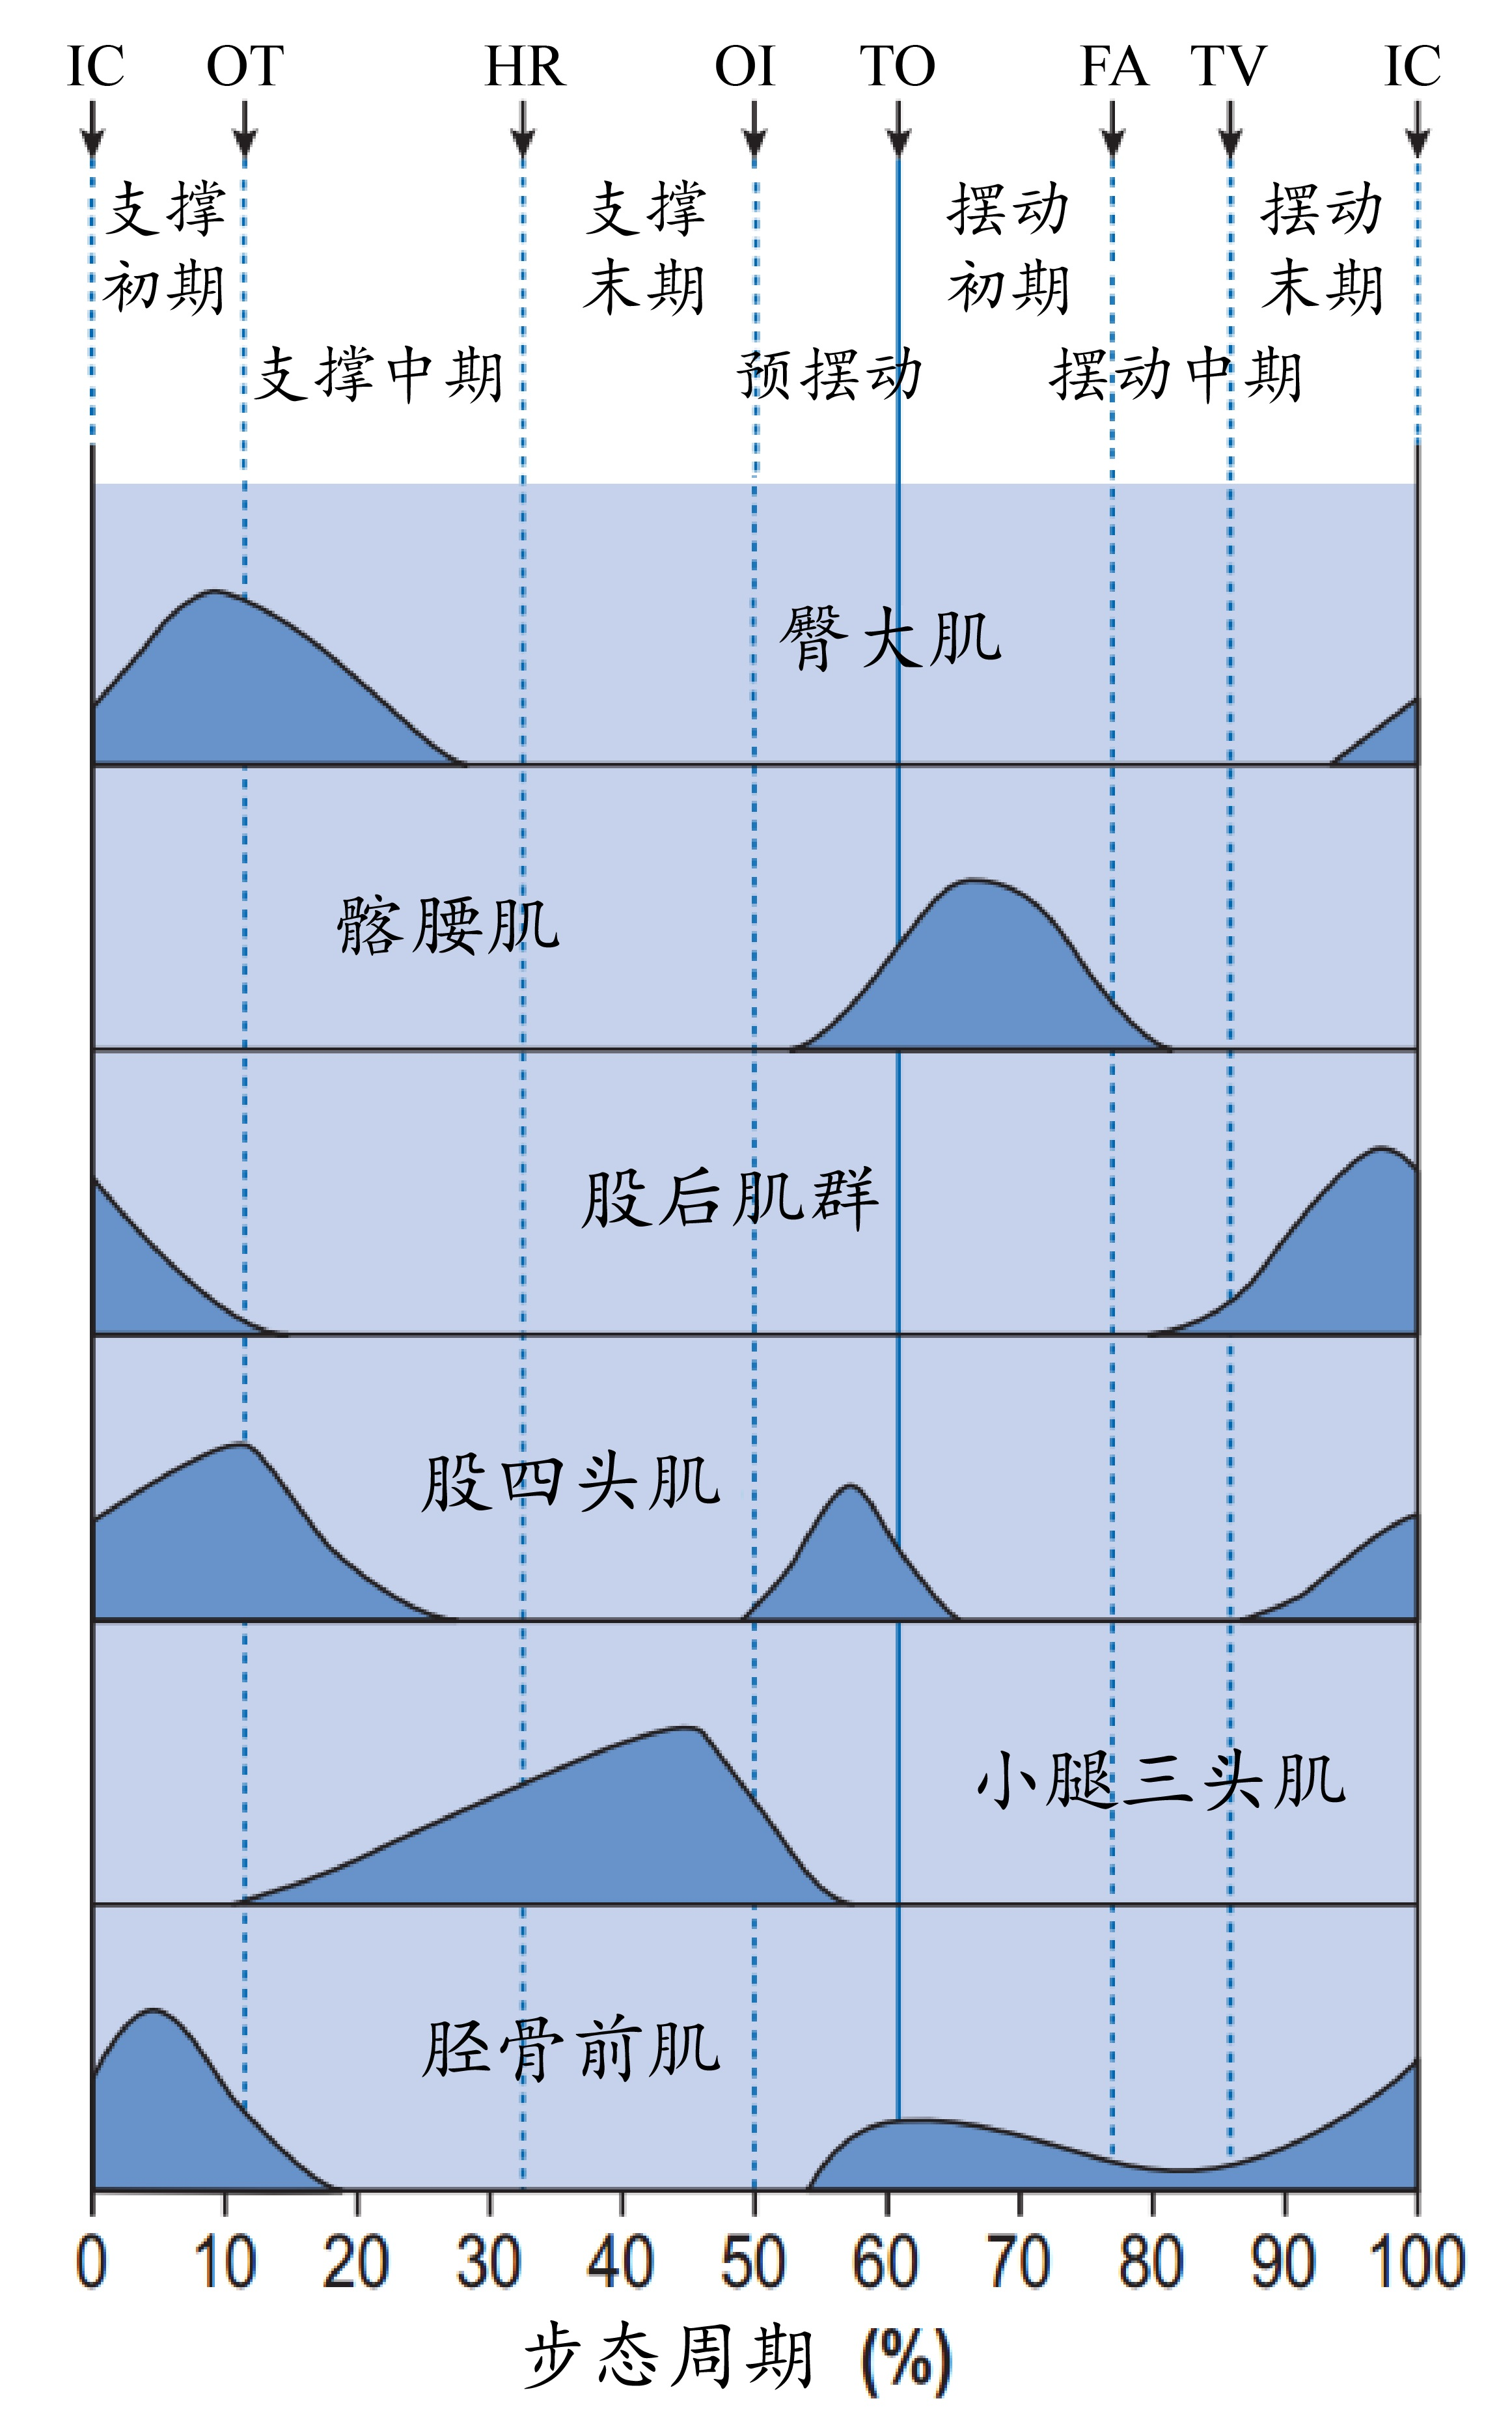
\includegraphics[width=8cm]{fig/f62.jpg}}
    \caption{步态过程的关节力矩与肌肉激活\cite{p44}}
    \label{fig:subfigss}
\end{figure}

行走时人体踝关节的运动主要受小腿三头肌和胫骨前肌控制,其中小腿三头肌由腓肠肌和比目鱼肌组成,控制髋关节拓屈,而胫骨前肌位于小腿前侧,控制髋关节背屈。比较图4.2中关节力矩曲线与肌肉激活度,可以看出小腿三头肌的收缩与踝关节力矩比较相似,而踝关节力矩与外骨骼助力紧密相关。因此可以考虑用肌肉的激活度来衡量穿戴者对助力模式的反应,若助力模式能够为人体提供有效辅助,则穿戴者的肌肉激活水平会随之而下降。

本文选择了腓肠肌内侧、比目鱼肌和胫骨前肌三块肌肉的每个周期激活度均方根之和作为肌肉激活指标进行生理信号反馈,其中肌肉的激活度由EMG信号经滤波后得到。为了确认所选择的生理反馈信号能够用于优化实验(在优化空间内具有明显的最小值),本文先对该生理反馈信号的有效性进行了验证,在优化参数空间内选择45个点进行采样,每个点的采样持续30s(约30个步态循环),之后对采集到的数据在参数空间内进行三维插值,得到目标函数关于优化参数的近似估计。如图4.3所示,肌肉激活指标以热力图的形式进行显示,图中蓝色区域表示肌肉激活水平较低,此区域的助力模式比较适合受试者。实验结果验证了肌肉激活指标作为生理反馈的有效性。
\begin{figure}[!htb]
    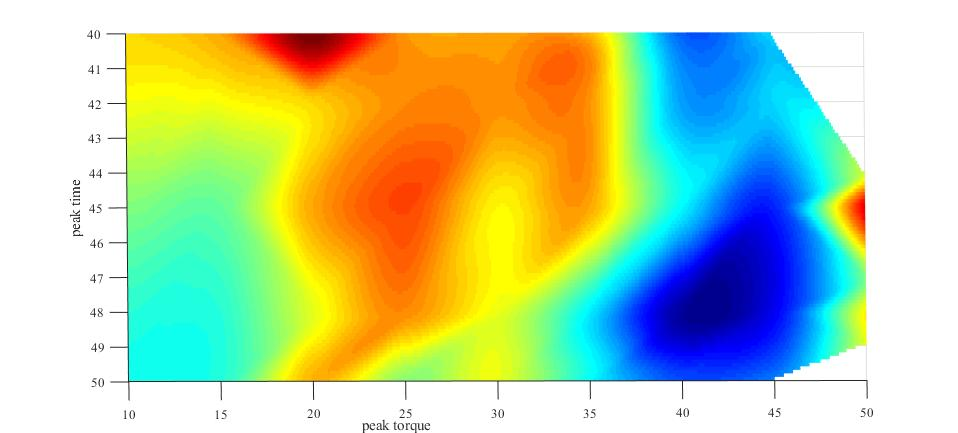
\includegraphics[width=17cm]{fig/f63.jpg}
    \caption{肌肉激活指标关于力矩参数近似估计}
    \label{fig:mark}
\end{figure}

\section{“人在环中”的外骨骼助力参数优化实验}

本文使用贝叶斯优化的方法,选择肌肉活跃度为生理反馈信号,对外骨骼力矩控制上层控制器的峰值力矩和峰值时间两个参数进行优化。

实验时受试者(本文作者)处于连续行走状态,每间隔15步进行一次优化迭代,每次迭代使用15步中最后5步肌肉活跃度的平均值作为生理反馈,更新最优估计并进行下一次迭代。优化迭代30次后认为优化收敛并停止优化,取30代的最优估计作为优化结果,即受试者的最优助力参数。优化完成后进行验证实验,分别记录受试者在外骨骼不施加辅助与施加最优助力参数下30步的肌肉激活水平。整个过程在相同实验条件下重复5次,每两次实验之间休息10分钟。
\begin{table}[htb]
    \caption[控制参数]{5次优化实验的最优助力参数}
    \begin{tabular}{llllll}
      \toprule
        峰值力矩 $N\cdot m$ & 43.8 & 46 & 43.6 & 47.6 & 44.6 \\
      \midrule
        峰值时间 $\%$ & 49.6 & 50 & 49.1 & 46.5 & 48.9 \\
      \bottomrule
    \end{tabular}
\end{table}

实验结果如表4.1和图4.4所示,峰值力矩分布在$45N\cdot m$左右,峰值时间分布在$49\% stride time$左右。优化结果与4.2小节的先验实验相一致,且符合受试者(本文作者)的主观感受。
\begin{figure}[htb]
    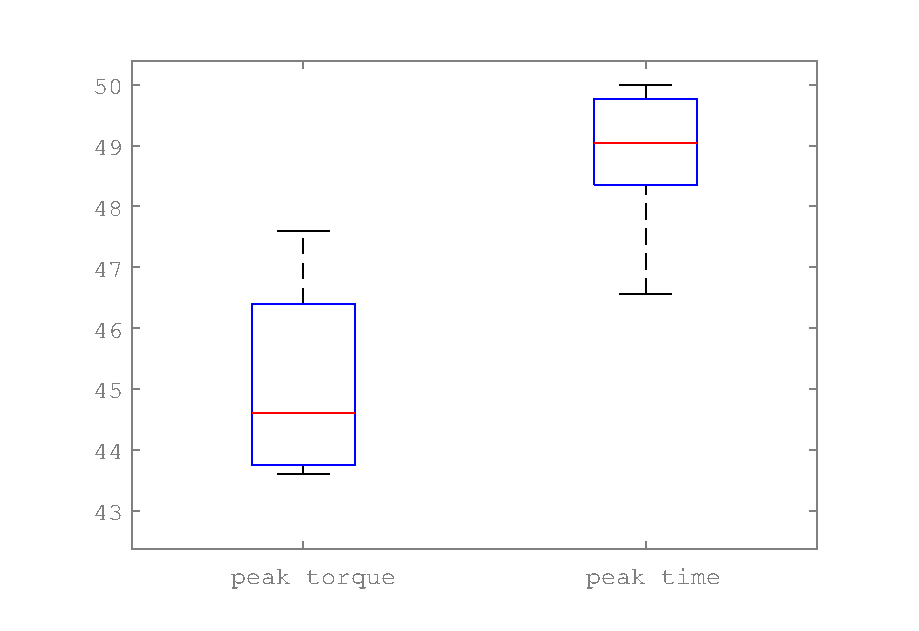
\includegraphics[width=11cm]{fig/f64.eps}
    \caption{最优助力参数的分布}
    \label{fig:mark}
\end{figure}
\begin{figure}[!htb]
    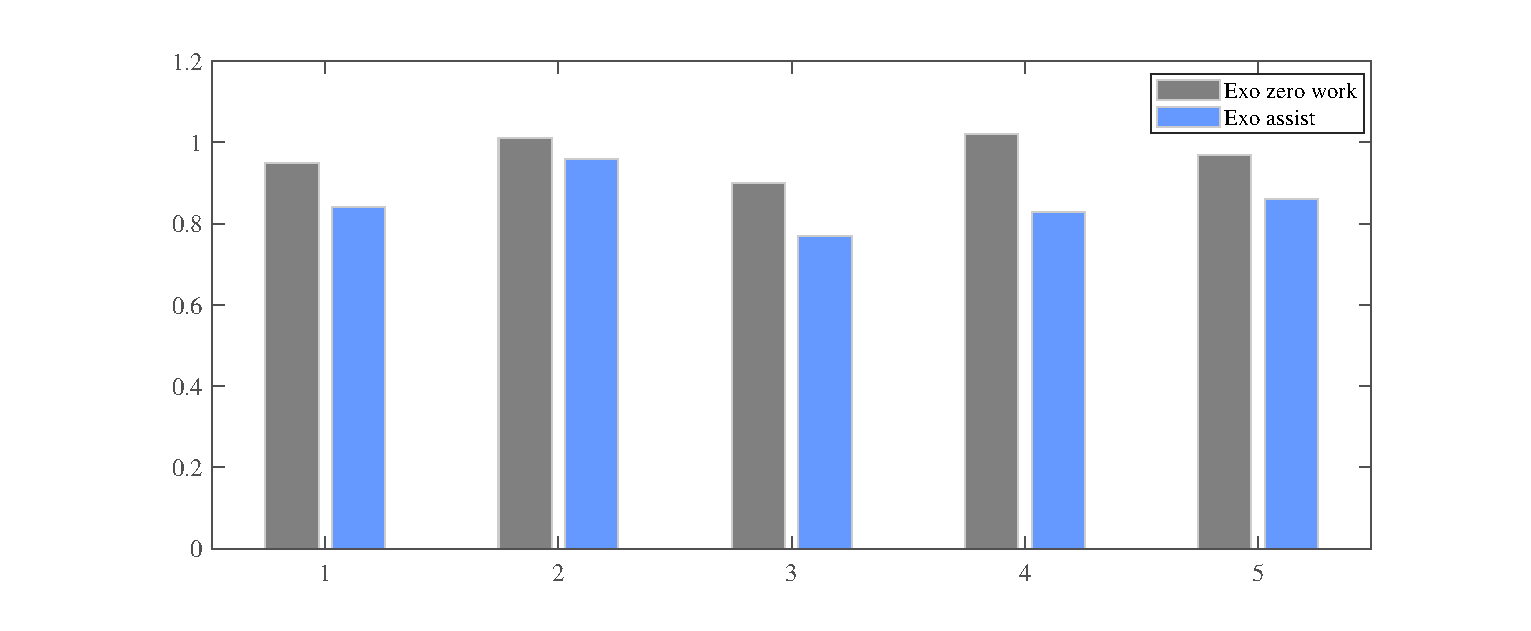
\includegraphics[width=17cm]{fig/f65.eps}
    \caption{最优助力参数的分布}
    \label{fig:mark}
\end{figure}
\begin{table}[!htb]
    \caption[控制参数]{优化参数下肌肉激活水平的下降程度}
    \begin{tabular}{cc}
      \toprule
      平均肌肉激活水平百分比 & 最大肌肉激活水平下降百分比 \\
      \midrule
        12.2\% & 18.6\% \\
      \bottomrule
    \end{tabular}
\end{table}

图4.5与表4.2显示了验证实验的结果。可以看出由优化得到的最优助力模式,均能够显著降低受试者的肌肉激活水平,其中平均肌肉激活水平下降12.2\%,最大下降18.6\%。

\section{本章小结}

本章针对外骨骼系统助力模式的调整问题,研究了“人在环中”的外骨骼参数优化方法。通过采集穿戴者对助力模式的生理反应,将其反馈至优化求解器中,不断迭代寻找最适合穿戴者的助力模式,从而充分发挥外骨骼潜能。实现上,本文采用贝叶斯优化方法,并选取基于EMG信号的肌肉激活指标作为生理反馈,通过实验验证了优化的有效性,并提高了时间效率。